\documentclass[]{article}
\usepackage[UTF8]{ctex}
\usepackage{graphicx}
\usepackage{appendix}
\usepackage{geometry}
\usepackage{amsmath}
\usepackage{cite}
\usepackage{natbib}
\usepackage{listings}
\usepackage{titlesec}
\usepackage{float}
\usepackage{enumitem}
\usepackage[labelfont=bf]{caption}
\usepackage{listings}
\usepackage{hyperref}
\usepackage[section]{placeins}
\usepackage{fix-cm}
\hypersetup{hidelinks,
	colorlinks=true,
	allcolors=black,
	pdfstartview=Fit,
	breaklinks=true
}

\lstset{
	basicstyle=\ttfamily,
	breaklines=true,
	frame=single,
	numbers=left,
	numberstyle=\tiny,
	language=[LaTeX]TeX
}

% Set ctex labels to English
\ctexset{
	contentsname = {Contents},
	figurename = {Figure},
	tablename = {Table},
	appendixname = {Appendix},
	abstractname = {Abstract},
	indexname = {Index},
	proofname = {Proof}
}

\begin{document}

\title{\huge Design of a LED controller}
\author{\large }
\date{}

\maketitle

\vspace{3cm}

\begin{center}
    {\large
        \begin{tabular}{|p{2.5cm}|p{3.5cm}|p{2.5cm}|p{3.5cm}|}
            \hline
            \textbf{Name}     &  & \textbf{Class} &       \\[0.8cm]
            \hline
            \textbf{Date}     &  & \textbf{Score} & \quad \\[0.8cm]
            \hline
            \textbf{Examiner} &  & \quad          & \quad \\[0.8cm]
            \hline
        \end{tabular}
    }
\end{center}

\newpage
\tableofcontents
\newpage
\newpage

\section{Introduction}
This experiment involves designing and implementing a digital LED controller using VHDL. The system is designed to control multiple LEDs through push-button inputs using an FPGA platform. The design employs state machines and counter logic to manage different LED patterns based on user input, demonstrating fundamental concepts in digital system design.

\section{Experiment procedure}

\subsection{Tools}
\begin{enumerate}[label = (\arabic*)]
    \item  Quartus II 13.0
    \item ModelSim
    \item Computer
    \item FPGA (clocking at 50MHz)
\end{enumerate}

\begin{figure}[H]
    \centering
    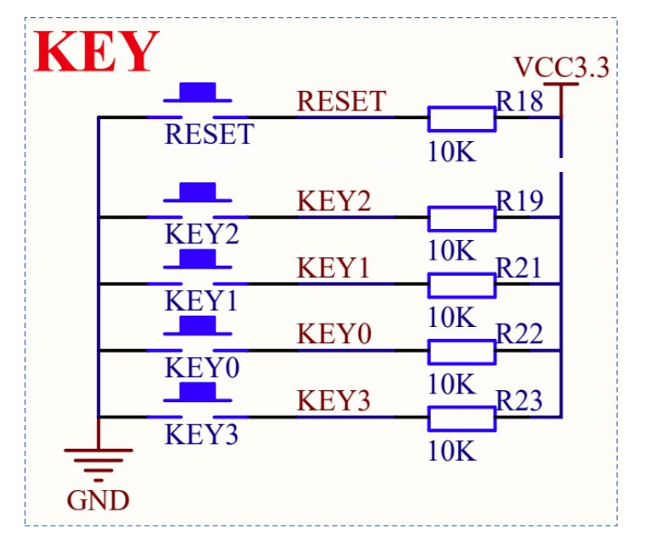
\includegraphics[width=0.85\linewidth]{first.png}
    \caption{System design}
    \label{sys}
\end{figure}
\subsection{The Project Overview}

\begin{enumerate}[label = (\arabic*)]
    \item Design the VHDL code to describe the LED
          controller. The controller has 4 control buttons and
          a reset button.
    \item  Design a testbench to test the function of the
          control system, by pressing the reset button and 4
          control buttons, respectively
    \item  Program the VHDL code to the FPGA and test its
          function by pressing the corresponding buttons.

\end{enumerate}

\noindent \textbf{The brief workflow are shown as figure\ref{flow} below}

\begin{figure}[H]
    \centering
    
\includegraphics[width=0.85\linewidth]{flow.png}
    \caption{Workflow}
    \label{flow}
\end{figure}
\subsection{LED control design}
\noindent \textbf{Below are our implement of the LEDs}

\begin{lstlisting}[language= VHDL]
LIBRARY IEEE;
USE IEEE.std_logic_1164.ALL;
USE IEEE.std_logic_unsigned.ALL;

entity key_ctrl is
port(sys_clk:in std_logic;
      sys_rst_n:in std_logic;
      key: in std_logic_vector(3 downto 0);
      led: out std_logic_vector(3 downto 0)
     );
end key_ctrl;

ARCHITECTURE Behavioral OF key_ctrl IS

signal cnt: std_logic_vector(23 downto 0);
signal led_control: std_logic_vector(1 downto 0);

BEGIN
process(sys_clk,sys_rst_n)
begin
if (sys_rst_n = '0') then
    cnt <= (others => '0');
elsif (rising_edge(sys_clk)) then
    if (cnt < "100110001001011001111111") then
    cnt <= cnt + 1;
    else
    cnt <= (others => '0');
    end if;
end if;

end process;
process(sys_clk,sys_rst_n)
begin
if (sys_rst_n = '0') then
    led_control <= "00";
elsif (rising_edge(sys_clk)) then
    if (cnt = "100110001001011001111111") then
    led_control <= led_control + 1;
    else
    led_control <= led_control;
    end if;
end if;
end process;

process(sys_clk, sys_rst_n)
begin
if (sys_rst_n='0') then
    led <= "0000";
elsif (rising_edge(sys_clk)) then
    if (key(0) = '0') then
        case led_control is
        when "00" =>
        led <= "1000";
        when "01" =>
        led <= "0100";
        when "10" =>
        led <= "0010";
        when "11" =>
        led <= "0001";
        when others =>
        led <= "0000";
        end case;
    elsif (key(1) = '0') then
        case led_control is
        when "00" =>
        led <= "0001";
        when "01" =>
        led <= "0010";
        when "10" =>
        led <= "0100";
        when "11" =>
        led <= "1000";
        when others =>
        led <= "0000";
        end case;
    elsif (key(2) = '0') then
        case led_control is
        when "00" =>
        led <= "1111";
        when "01" =>
        led <= "0000";
        when "10" =>
        led <= "1111";
        when "11" =>
        led <= "0000";
        when others =>
        led <= "0000";
        end case;
    elsif (key(3) = '0') then
        led <= "1111";
    else
        led <= "0000";
    end if;
end if;
end process;
 
END Behavioral;

\end{lstlisting}

\begin{figure}[H]
    \centering
    
\includegraphics[width=0.85\linewidth]{vhd.png}
    \caption{LED Controller Implementation}
    \label{vhd}
\end{figure}

\subsection{Testbench Design}
\renewcommand{\theenumi}{(\arabic{enumi})}

\noindent \textbf{Below are our implement of the testbench}\\

\begin{lstlisting}[language=VHDL]
LIBRARY ieee;                                               
USE ieee.std_logic_1164.all;                                

ENTITY key_ctrl_vhd_tst IS
END key_ctrl_vhd_tst;
ARCHITECTURE key_ctrl_arch OF key_ctrl_vhd_tst IS
-- constants                                                 
-- signals                                                   
SIGNAL key : STD_LOGIC_VECTOR(3 DOWNTO 0);
SIGNAL led : STD_LOGIC_VECTOR(3 DOWNTO 0);
SIGNAL sys_clk : STD_LOGIC;
SIGNAL sys_rst_n : STD_LOGIC;
CONSTANT clk_period : time := 20ns;
COMPONENT key_ctrl
    PORT (
    key : IN STD_LOGIC_VECTOR(3 DOWNTO 0);
    led : OUT STD_LOGIC_VECTOR(3 DOWNTO 0);
    sys_clk : IN STD_LOGIC;
    sys_rst_n : IN STD_LOGIC
    );
END COMPONENT;
BEGIN
    i1 : key_ctrl
    PORT MAP (
-- list connections between master ports and signals
    key => key,
    led => led,
    sys_clk => sys_clk,
    sys_rst_n => sys_rst_n
    );
clk_gen : process 
begin
    sys_clk <= '1';
    wait for clk_period/2;
    sys_clk <= '0';
    wait for clk_period/2;
end process;
init : PROCESS                                               
-- variable declarations                                     
BEGIN                                                        
       key <= "1111";
    sys_rst_n <= '0';
    wait for 400ms;
    sys_rst_n <= '1';
    wait for 200ms;
    key(0) <= '0';
    wait for 800ms;
    key(0) <= '1';
    key(1) <= '0';
    wait for 800ms;
    key(1) <= '1';
    key(2) <= '0';
    wait for 800ms;
    key(2) <= '1';
    key(3) <= '0';
    wait for 800ms;
    key(3) <= '1';                      
WAIT;                                                       
END PROCESS init;                                           
always : PROCESS                                              
-- optional sensitivity list                                  
-- (        )                                                 
-- variable declarations                                      
BEGIN                                                         
        -- code executes for every event on sensitivity list  
WAIT;                                                        
END PROCESS always;                                          
END key_ctrl_arch;

\end{lstlisting}

\begin{figure}[H]
    \centering
    
\includegraphics[width=0.85\linewidth]{vht.png}
    \caption{Testbench Implementation}
    \label{vht}
\end{figure}


\subsection{Programming the FPGA}
\noindent \textbf{Assignment pin planner}

\begin{figure}[h]
    \centering
    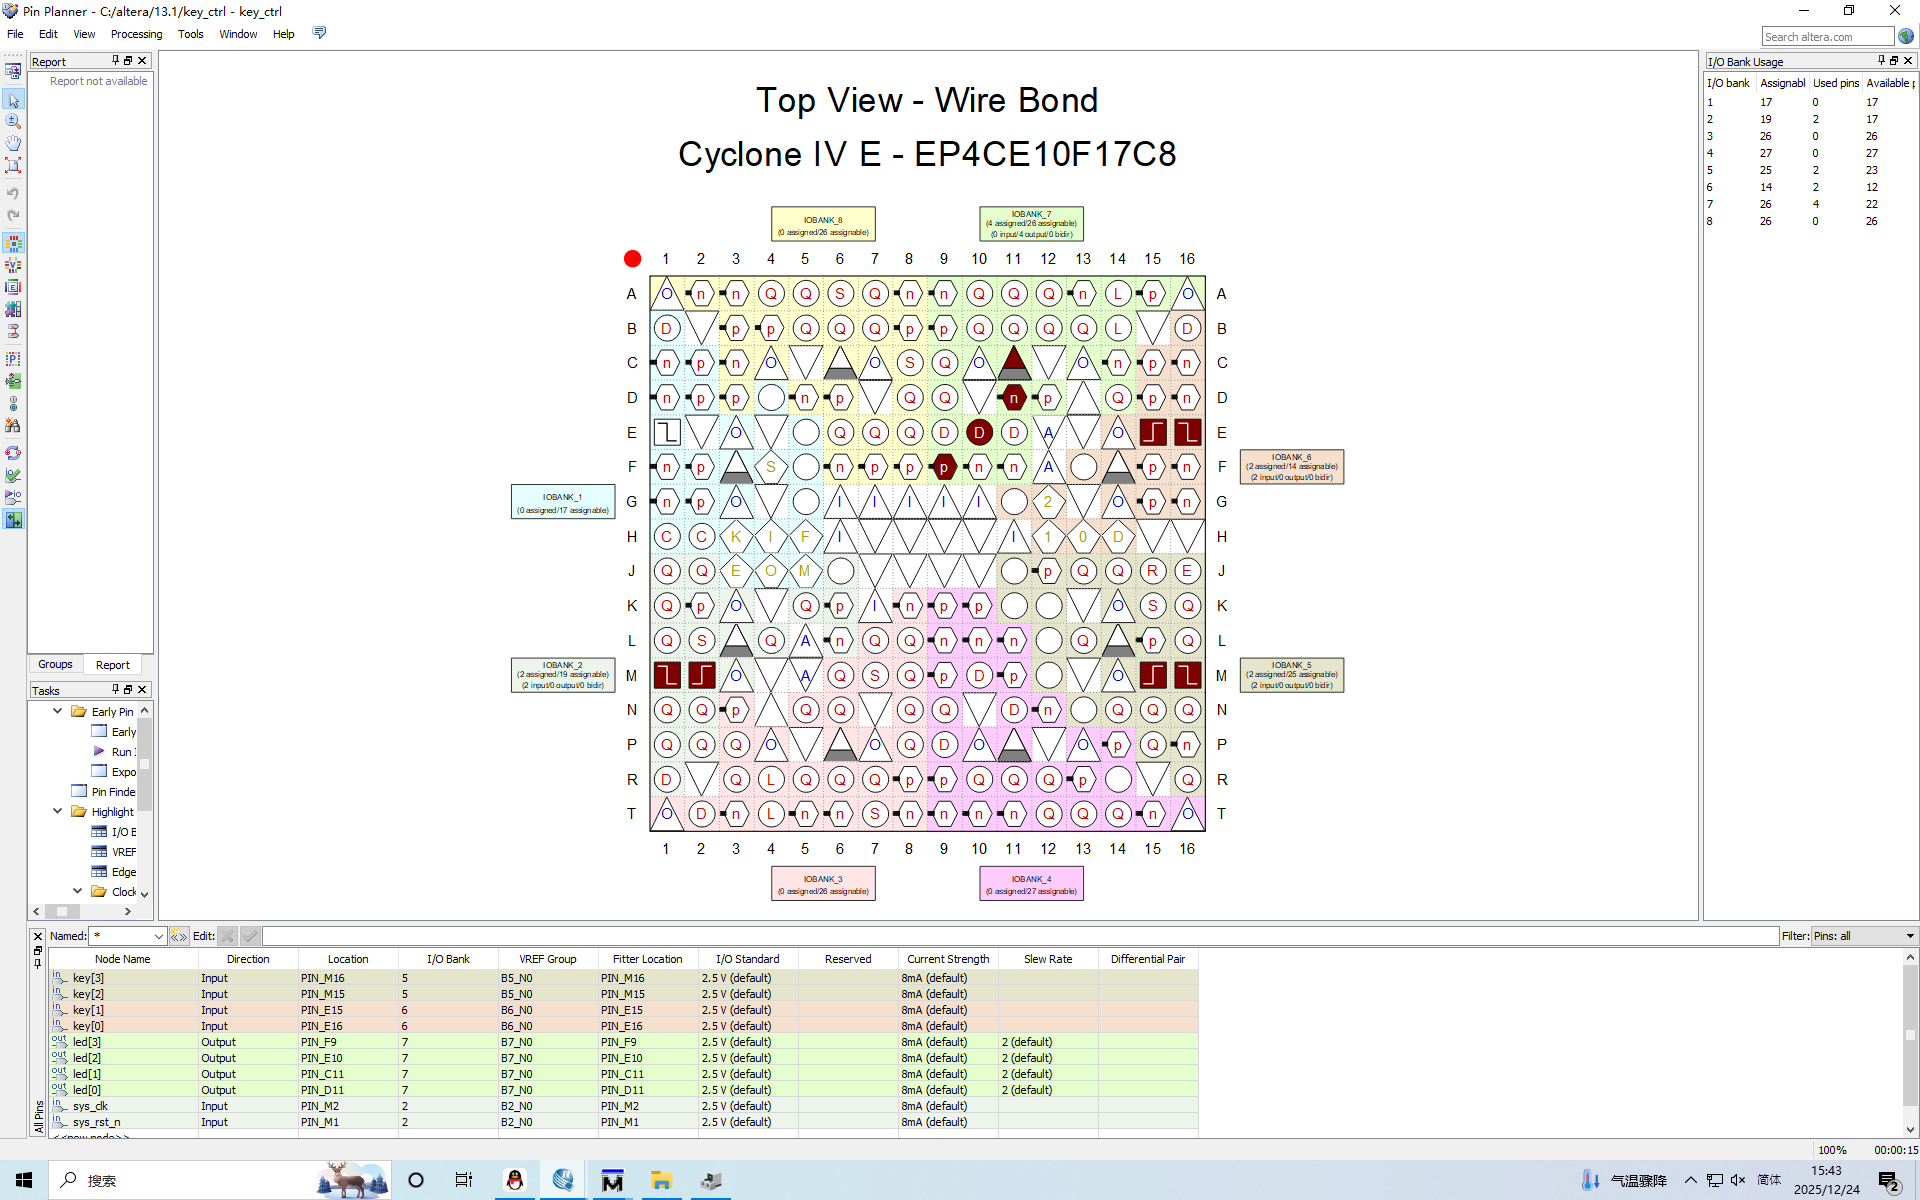
\includegraphics[width=0.85\linewidth]{pin3.png}
    \caption{Pin assignment}
    \label{pin}
\end{figure}

\begin{figure}[h]
    \centering
    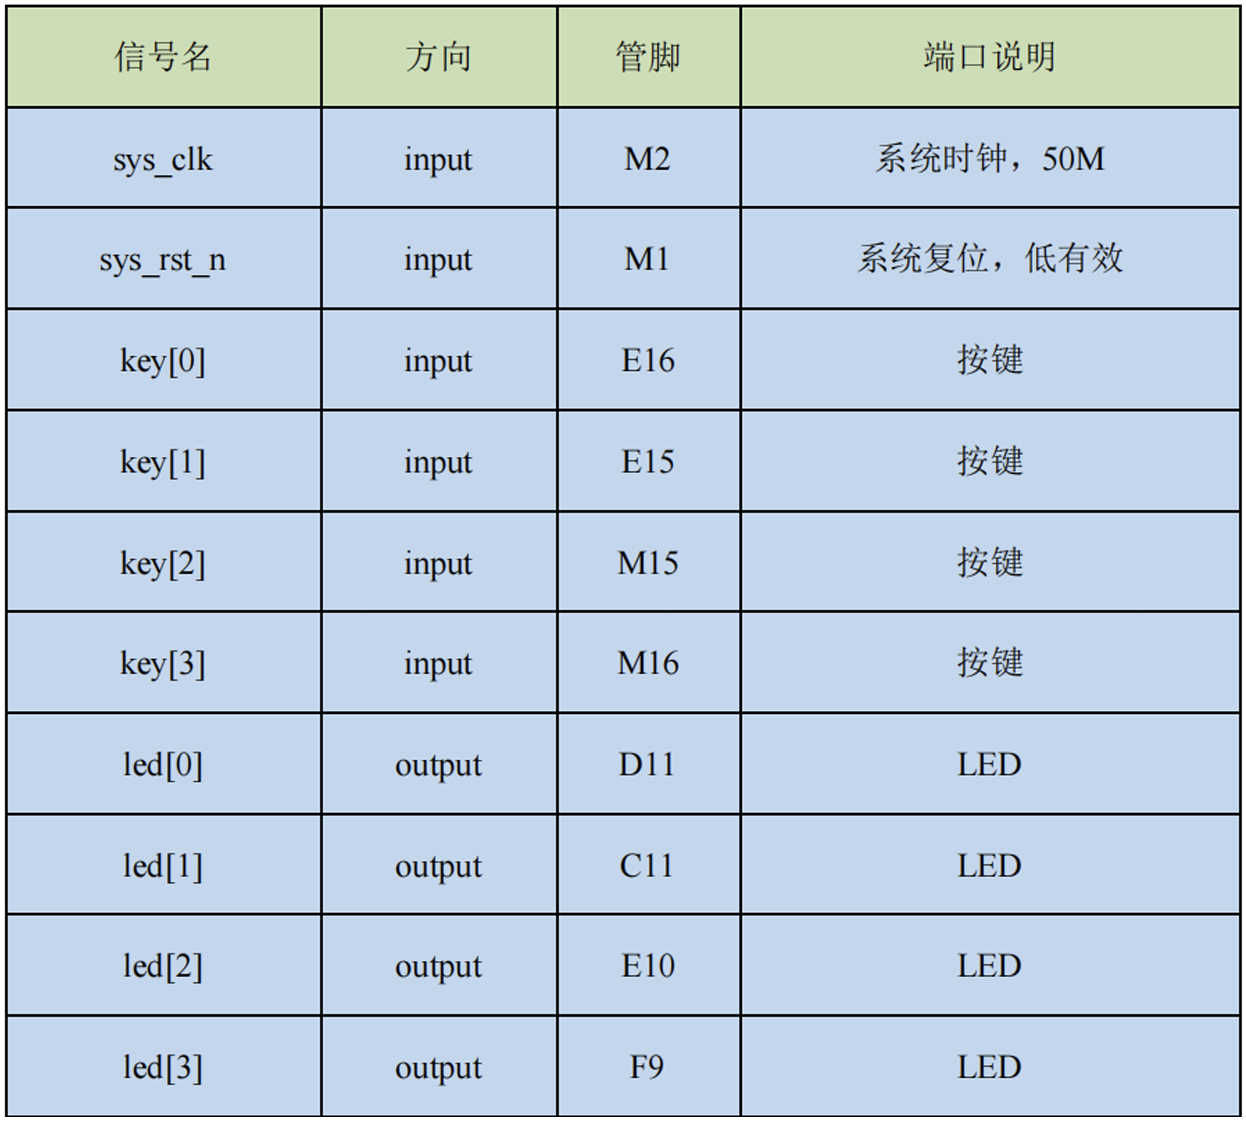
\includegraphics[width=0.85\linewidth]{assignment.jpg}
    \caption{Pin assignment}
    \label{pin}
\end{figure}

% \noindent \textbf{ Download verification and comply with it in FPGA}

\subsection{Waveform}
\begin{figure}[H]
    \centering
    
\includegraphics[width=0.85\linewidth]{wave.png}
    \caption{Simulation Of The Waveform}
    \label{wave}
\end{figure}
\subsection{FPGA experiment}

\begin{figure}[H]
    \centering
    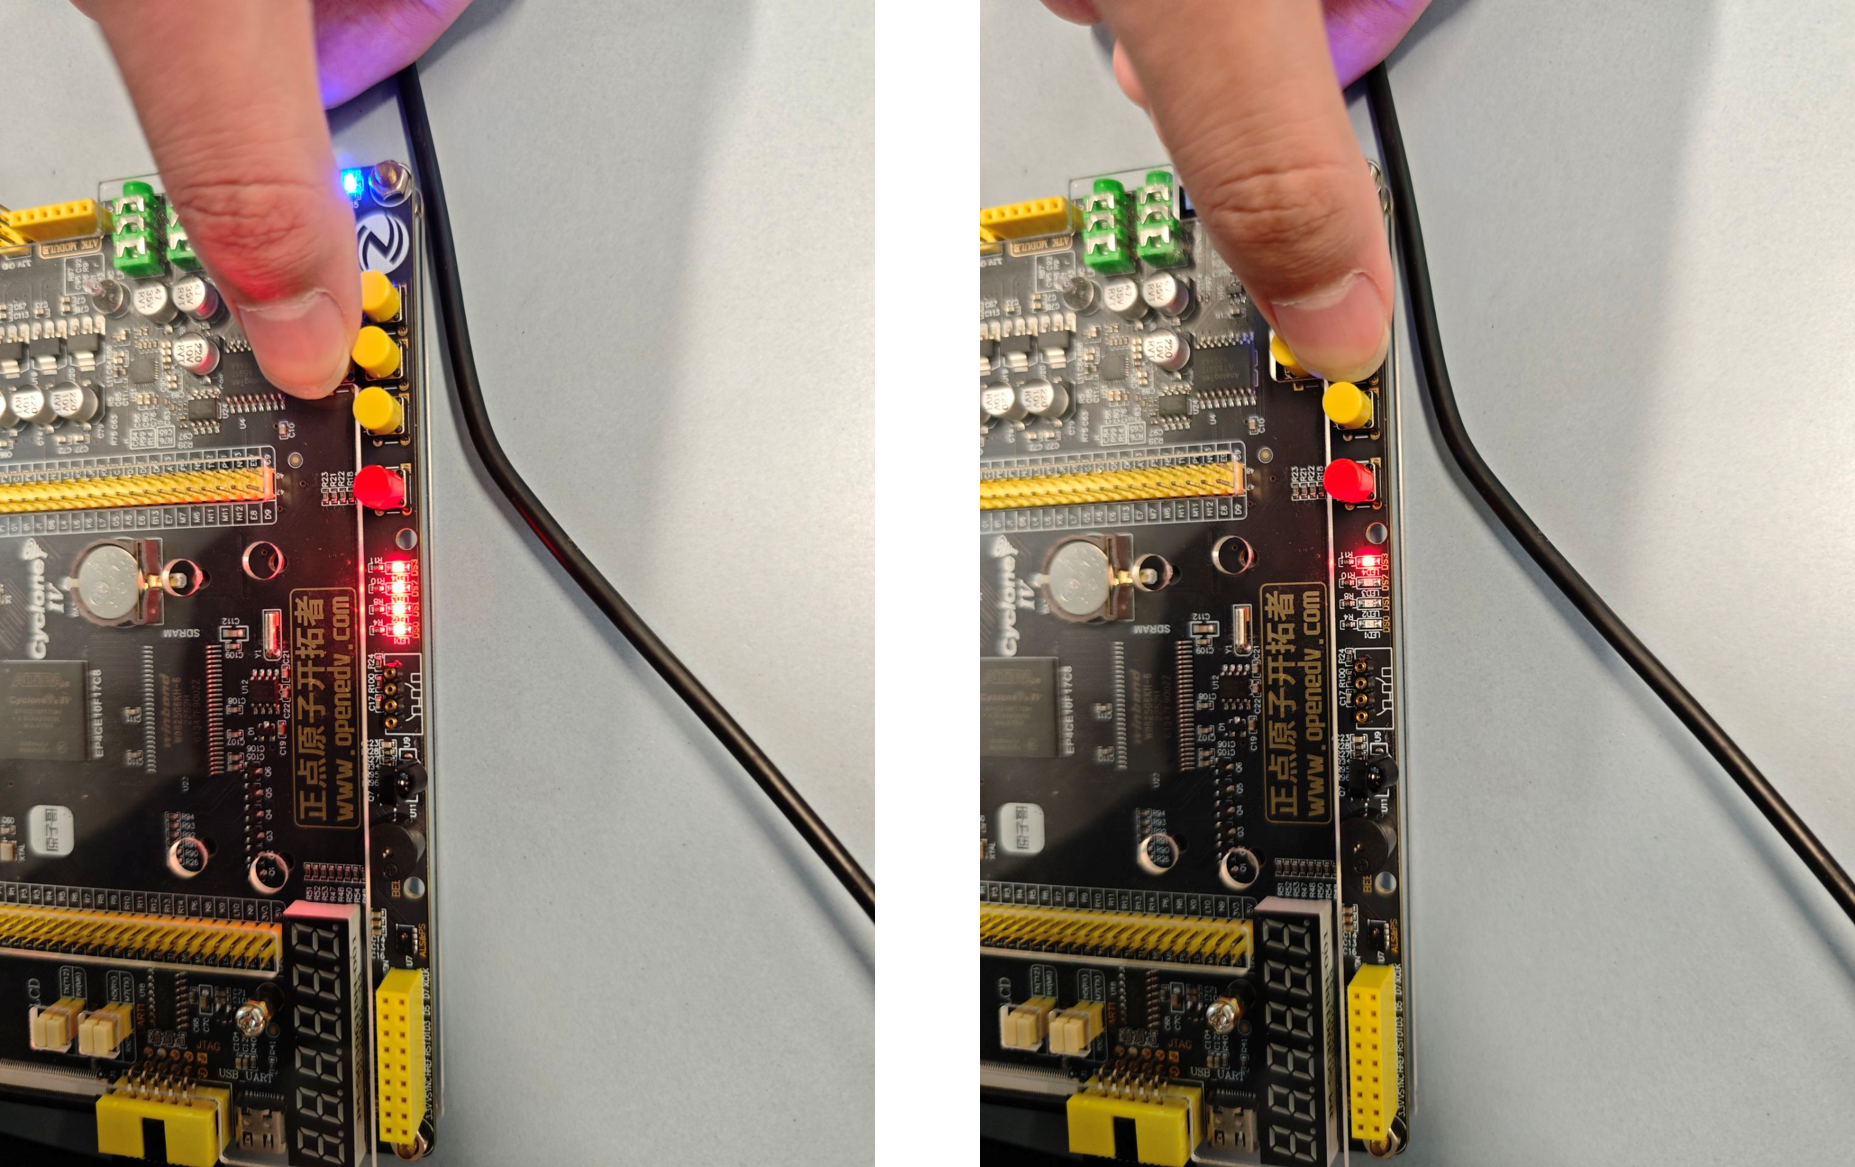
\includegraphics[width=0.85\linewidth]{p1.png}
    \caption{FPGA experiment}
\end{figure}
\section{Analysis and discussion}

\subsection{System Design and Functionality}

The system designed in this experiment is a simple yet effective digital circuit that controls four LEDs based on the state of four push-button switches. The system operates under the control of a clock signal (\texttt{sys\_clk}) and a reset signal (\texttt{sys\_rst\_n}). The behavior of the LEDs is determined by the state of the buttons (\texttt{key}) and a counter (\texttt{cnt}) that generates a timing signal to control the LED patterns.

\subsubsection{Reset Functionality}
When the reset button is pressed (\texttt{sys\_rst\_n} = '0'), the system resets to its initial state, turning off all LEDs (\texttt{led} = "0000"). This ensures that the system starts from a known state, which is crucial for reliable operation.

\subsubsection{Button-Controlled LED Patterns}
\begin{itemize}
    \item \textbf{Button key(0) (Right-to-Left Flow):} When \texttt{key(0)} is pressed, the LEDs light up in a sequence from right to left (\texttt{led(3)} to \texttt{led(0)}). This pattern is achieved by incrementing a 2-bit control signal (\texttt{led\_control}) that determines the current LED state.
    \item \textbf{Button key(1) (Left-to-Right Flow):} When \texttt{key(1)} is pressed, the LEDs light up in a sequence from left to right (\texttt{led(0)} to \texttt{led(3)}). This pattern is also controlled by the \texttt{led\_control} signal, but the sequence is reversed.
    \item \textbf{Button key(2) (Blinking):} When \texttt{key(2)} is pressed, the LEDs blink on and off in a repeating pattern. This effect is achieved by toggling the LEDs on and off based on the \texttt{led\_control} signal.
    \item \textbf{Button key(3) (All LEDs On):} When \texttt{key(3)} is pressed, all LEDs are turned on (\texttt{led} = "1111"). This is a simple state where no pattern is involved, and all LEDs remain on.
    \item \textbf{No Button Pressed:} When no button is pressed, the LEDs remain off (\texttt{led} = "0000").
\end{itemize}

\subsubsection{Timing Control}
The system uses a 24-bit counter (\texttt{cnt}) to generate a timing signal. The counter increments on each rising edge of the clock (\texttt{sys\_clk}) and resets to zero when it reaches a specific value ("10011000100101101111111"), which corresponds to a delay of approximately 0.2 seconds at a 50 MHz clock frequency. This timing signal is used to control the interval between LED state changes, ensuring that the patterns are displayed at the desired rate.

\subsection{Testbench Design and Simulation}

The testbench is designed to verify the functionality of the system by simulating the behavior of the push-button switches and observing the corresponding LED patterns. The testbench includes the following features:

\subsubsection{Reset Test}
The testbench first checks the reset functionality by pressing the reset button and verifying that all LEDs turn off.

\subsubsection{Button Press Tests}
The testbench simulates pressing each of the four buttons (\texttt{key(0)} to \texttt{key(3)}) and verifies that the LEDs display the correct patterns:
\begin{itemize}
    \item \textbf{Button key(0) (Right-to-Left Flow):} The LEDs should light up in sequence from right to left.
    \item \textbf{Button key(1) (Left-to-Right Flow):} The LEDs should light up in sequence from left to right.
    \item \textbf{Button key(2) (Blinking):} The LEDs should blink on and off in a repeating pattern.
    \item \textbf{Button key(3) (All LEDs On):} All LEDs should remain on.
\end{itemize}

\subsubsection{No Button Press Test}
The testbench also checks the behavior when no button is pressed, ensuring that all LEDs remain off.

\subsubsection{Timing Verification}
The testbench verifies that the interval between LED state changes is approximately 0.2 seconds, as expected.

\subsubsection{Simulation Results}
The simulation results show that the system behaves as expected, with the LEDs displaying the correct patterns based on the state of the buttons. The timing of the LED patterns is also verified to be accurate.

\subsection{FPGA Programming and Testing}

The FPGA programming process involves several key steps:

\subsubsection{Pin Assignment}
The Assignment-Pin Planner is used to allocate the pins properly, ensuring that the inputs (buttons) and outputs (LEDs) are correctly mapped.

\subsection{Challenges and Solutions}

\subsubsection{Timing Issues}
One of the challenges in this experiment was ensuring that the timing of the LED patterns was accurate. The 24-bit counter was designed to generate a timing signal every 0.2 seconds, but slight variations in the clock frequency could affect the timing. To address this, the counter value was carefully calculated to ensure that the timing was within the desired range.

\subsubsection{Button Debouncing}
Another challenge was dealing with button debouncing, which can cause unintended state changes when a button is pressed. To mitigate this, the system was designed to ignore short-duration button presses, ensuring that only stable button presses are recognized.

\subsubsection{Testbench Verification}
Writing a comprehensive testbench was challenging, especially when simulating the timing of the LED patterns. The testbench was designed to include all possible inputs and verify the system's behavior under different conditions. The use of ModelSim for waveform simulation helped in visualizing the system's behavior and verifying its correctness.

\section{Conclusion and self-review}
\noindent The experiment successfully demonstrates the design and implementation of a digital system that controls four LEDs using four push-button switches. The system is developed in VHDL and tested using a testbench in ModelSim. The FPGA is programmed to display various LED patterns based on the state of the buttons, with its functionality verified through both simulation and physical testing. This experiment emphasizes the critical roles of timing control, button debouncing, and thorough testing in the design of digital systems. The results confirm that the system performs as expected, with the LEDs displaying the correct patterns corresponding to the button states. The use of VHDL and ModelSim provides a solid framework for designing and testing digital systems, making it an invaluable tool for future projects.
\end{document}
